\section{Introduction} 

Rapidly exploring Random Trees (RRT) is a path planning algorithm which explores
a space by building a tree of random possible moves.
Each branch is built by extending in a random direction that does result in a collision.
The length of the attempted extension is a general RRT parameter called \(\epsilon\)
\citep{pathplanning}.

The bidirectional RRT is a method which builds two trees,
one from a goal position, and one from a starting position.
When the trees meet each other, a path can be found as a series of steps
from the root of one tree to the root of the other.

The balanced bidirectional RRT is a method which ensures that both trees are of the same size. 
This method is good for getting out of traps where there is plenty of space in the wrong directions.

A simulated KukaKr16 robot \citep{kukakr16} is given the task of picking
up a bottle from a crate and placing it on a table in an environment
generated using the RobWork \citep{robwork} framework.
The workspace is confined by a wall, so the robot has to spin
around itself in order to reach the goal. This presents a path planning
challenge, as it may be desirable to keep the distance traveled by the robot
as small as possible. Note that in terms of energy requirements,
it may be desirable to minimize the jointspace distance traveled, and not the
euclidean distance traveled by the bottle.
The simulated setup can be seen in figure \ref{fig:worckcell_bottle_picked}.

\begin{figure}[h]
 \centering
 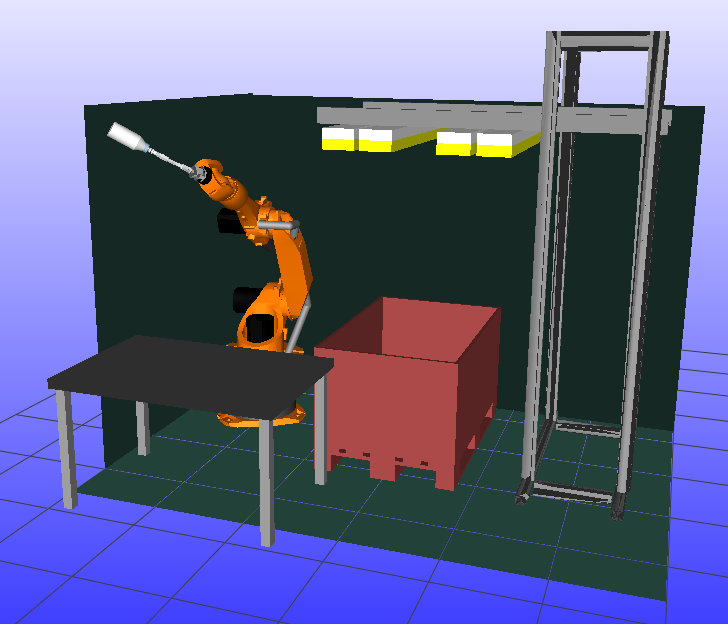
\includegraphics[width=\figsize]{graphics/robworkpic}
 \caption{RobWork simulation workcell with KukaKr16 robot.
 The RRT algorithms are applied to the problem of moving the bottle
 in a collision-free path from the red box to the table.}
 \label{fig:worckcell_bottle_picked}
\end{figure}

The RRT planners takes a parameter \(\epsilon\),
which is a measure of the aggressiveness of the algorithm.
To evaluate the performance of the algorithm,
the jointspace path length \(d_J\) is calculated.
Since the space is explored in random directions,
the path length will not be the same in every trial.
Thus, to evaluate the algorithm performance, several trials are made,
in which the starting and goal positions are the same,
and in which the RRT planner is reset every time.

A first hypothesis is that \(\epsilon\) is correlated with the
jointspace path length \(d_J\) and thus that an optimal \(\epsilon\) exists
for the given configuration and algorithm. The null-hypthesis
\(H_{0,corr}\) is that \(\epsilon\) is not correlated with \(d_J\).

For each algorithm, the optimal value of this parameter is found
with respect to the total joint space distance traveled by the simulated serial robot.
Thus, if indeed an optimal \(\epsilon\) exists for each algorithm,
it can be shown whether or not one finds shorter paths than the other.
It is hypothesized that one algorithm will find shorter paths than the other.
The null-hypothesis \(H_{0,comp}\) is that the algorithms yield
the same path lengths \(d_J\). The alternate hypothesis \(H_{1,comp}\)
is that one algorithm yields shorter path lengths \(d_J\) than the other.